\documentclass{cubeamer}

\title{Ethische Risiken und Chancen von CoEnv}
\subtitle{Endpräsentation Global Citizenship}
\author[Kay Schuh, Max Richter]{Kay Schuh, Max Richter}
\date{\today} % or whatever the date you are presenting in is
\institute[Technische Hochschule Köln]{Code \& Context}
% \copyrightnotice{Published by the American Institute of Aeronautics and Astronautics, Inc., with permission}

\usepackage{quoting}


\begin{document}

\maketitle

% \cutoc

\section{Einleitung}

\begin{frame}{Symbolsprache}
    \begin{center}
    \includesvg[height = 0.7\textheight]{img/sigil}
    \end{center}
\end{frame}

\section{Ethische Fragestellung}
\begin{frame}{Die Triskele}
    \begin{columns}
        \begin{column}{0.6\textwidth}
            \begin{figure}
                \centering
                \includesvg[height = 0.7\textheight]{img/triskele}
                \caption{\tiny AnonMoos, Public Domain, via Wikimedia Commons}
            \end{figure}
        \end{column}
        \begin{column}{0.4\textwidth}
            \begin{itemize}
                \item Jungsteinzeit
                \item In fast allen Kulturen vertreten
                \item Bedeutet "Weg des Lebens"
                \item Rollenverteilung innerhalb des BDSMs
                \only<2->{\item Benutzung durch rechtsextreme Gruppierung}
            \end{itemize}
        \end{column}
    \end{columns}
\end{frame}

\begin{frame}{Rechtsextremer Kontext}
    \begin{columns}
        \begin{column}{0.6\textwidth}
            \begin{figure}
                \centering
                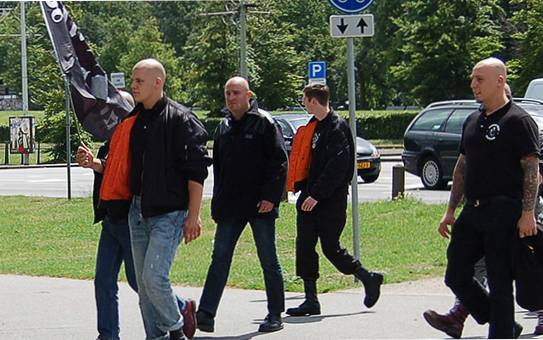
\includegraphics[height = 0.5\textheight]{img/bah.jpg}
                \caption{\tiny Demonstration von Blood \& Honour-Aktivisten in Den Haag, Juni 2011. / Wouter Engler (CC BY-SA 4.0 cropped)}
            \end{figure}
        \end{column}
        \begin{column}{0.4\textwidth}
Blood and Honour ist ein rechtsextremes Netzwerk, das neonazistische Bands miteinander  koordiniert und die nationalsozialistische Ideologie verbreitet. Weltweit ist von bis zu 10.000 Mitgliedern auszugehen.
        \end{column}
    \end{columns}
\end{frame}

\begin{frame}{Was ist Three Seven?}
    \begin{columns}
        \begin{column}{0.6\textwidth}
            \begin{figure}
                \includesvg[height = 0.7\textheight]{img/three_seven_red}
                \caption{\tiny Von WarX, CC BY-SA 3.0, commons.wikimedia.org/w/index.php?curid=548112}
            \end{figure}
        \end{column}
        \begin{column}{0.4\textwidth}
            \begin{figure}
                \includesvg[height=0.6\textheight]{img/three_seven_sigil}
            \end{figure}
        \end{column}
    \end{columns}
\end{frame}

\begin{frame}{Was ist Elhaz?}
    \begin{columns}
        \begin{column}{0.6\textwidth}
            \begin{figure}
                \includesvg[height = 0.7\textheight]{img/elhaz}
                \caption{\tiny Von WarX, CC BY-SA 3.0, commons.wikimedia.org/w/index.php?curid=548112}
            \end{figure}
        \end{column}
        \begin{column}{0.4\textwidth}
            \only<1>{\begin{itemize}
                \item Die "Lebensrune"
                \item Eibe
                \item Unicode U+16C9
                \item Von den Nationalsozialisten als Geburtssymbol benutzt
            \end{itemize}}
            \only<2->{
                \begin{figure}
                    \includesvg[height = 0.7\textheight]{img/elhaz_sigil}
                \end{figure}
            }
        \end{column}
    \end{columns}
\end{frame}

\begin{frame}
    % Kontext: Personen wissen um den Kontext des Zeichens
    \huge Sollen wir den Gebrauch dieses Symbols in CoEnv technisch verbieten?
     \only<2->{
    \\[2ex]
        \normalsize Beide? Nur Elhaz? Nur die Triskele? Keins?
    }
\end{frame}

\section{Erläuterung}

\begin{frame}{Paragraph 86a Strafgesetzbuch}
\begin{enumerate}
    \item im Inland Kennzeichen einer der in [...] bezeichneten Parteien oder Vereinigungen verbreitet oder öffentlich [...] oder
    \item einen Inhalt [...], der ein derartiges Kennzeichen darstellt [...] zur Verbreitung oder Verwendung im Inland oder Ausland in der in Nummer 1 bezeichneten Art und Weise herstellt, vorrätig hält, einführt oder ausführt.
\end{enumerate}
\end{frame}

\begin{frame}{Paragraph 86a Absatz 3}
    3. Absatz 1 gilt nicht, wenn die Handlung der staatsbürgerlichen Aufklärung, [...], der \textbf{Forschung oder der Lehre}, der Berichterstattung über Vorgänge des Zeitgeschehens oder der Geschichte oder ähnlichen Zwecken dient.
\end{frame}

\section{Sachanalyse}


\begin{frame}{Sach-Analyse}
    \hfuzz=500pt
    tiny{\begin{tabular}[h]{l|c|c|r}
        Akteure  & \textbf{Interesse} & \textbf{Ziel} & \textbf{Mittel} \\
        \hline
        Leitende Personen & Entscheidung über Nutzung und Equipment des Workspaces & Effiziente und zufriendenstellende Nutzung & Bedachte Nutzung der Arbeitsplätze und Geldmittel \\
        \hline
        Gäste & Halten sich am geteilten Workspace auf & Sich ohne Konflikte dort zurechtfinden & Informationen von CoEnv und dessen Nutzern \\
        \hline
        Nutzer & Nutzen das CoEnv aktiv & Effizientes Zurechtfinden im Arbeitsumfeld & Verständigung über das CoEnv \\ 
        \hline
        Entwickler & Das Team hinter CoEnv & Erfolg mit CoEnv und dem Studium & Entwicklung und Etablierung des CoEnv
    \end{tabular}}
\end{frame}

\begin{frame}{Werte-Analyse}
    \small{\begin{center}
        \begin{tabular}[h]{l|c}
              & \textbf{Werte} \\
            \hline
            Leitende Personen & Funktionsfähigkeit, Wirtschaftlichkeit \\
            \hline
            Gäste & Gesellschaftsqualität, Sicherheit, Funktionsfähigkeit \\
            \hline
            Nutzer & Persönlichkeitsentfaltung, Sicherheit, Funktionsfähigkeit, Gesundheit \\ 
            \hline
            Entwickler & Wirtschaftlichkeit, Funktionsfähigkeit, Persönlichkeitsentfaltung
        \end{tabular}
    \end{center}}
\end{frame}

\begin{frame}{Resultierende Werte-Konflikte}
    \begin{center}
        \begin{tabular}{ r c l }
         Persönlichkeitsentfaltung & \(\Leftrightarrow\) & Glück \\
         \only<2->{Freiheit & \(\Leftrightarrow\) & Sicherheit}
        \end{tabular}
    \end{center}
\end{frame}

\section{Ethische Fragestellung 2.0}

\begin{frame}
   \large Eine Person will die Triskele nutzen für ein Projekt nutzen, weil sie sich gerne mit der keltischen Geschichte befasst. Sollen wir die Nutzung erlauben?
\end{frame}

\begin{frame}{Begründung\&Antwort Max}
    \begin{itemize}
        \item Positive Kausalverantwortung
        \item Utilitaristisch, der verursachte Schmerz wäre größer als das Glück der gewonnenen Freiheit
        \item Maximalprinzip
        \begin{itemize}
            \item Nur ausgewählte Symbole erlauben \(\Rightarrow\) Sicherheit
            \item Alles erlauben \(\Rightarrow\) Freiheit
        \end{itemize}
        \only<2->{\item[\(\hookrightarrow\)] \textbf{Übernehmen der Liste verbotener Zeichen nach \S 86a.}}
    \end{itemize}
\end{frame}

\begin{frame}{Begründung\&Antwort Kay}
    \begin{itemize}
        \item Angehörige von Opfern verbinden Symbol womöglich nicht direkt mit Schmerz, sondern durch abweichende Verwendung als neutral oder positiv
        \item Pflichtethik (nach Immanuel Kant)
        \begin{itemize}
            \item Die freie Meinungsäußerung ist ein Grundwert und würde direkt eingeschränkt
            \item Freie Nutzung steht über möglichen Konsequenzen \(\Rightarrow\) Freiheit, Gerechtigkeit
        \end{itemize}
        \item Negativer Utilitarismus
        \begin{itemize}
            \item Nutzer von CoEnv büßen aus Rücksicht Freiheit ein 
            \item Filter gegen die Triskele \(\Rightarrow\) Sicherheit, Glück
        \end{itemize}
        \only<2->{\item[\(\hookrightarrow\)] \textbf{Die abstrakten Symbole bedürfen keines zusätzlichen Filters.}}
    \end{itemize}
\end{frame}


% Q&A
\begin{frame}[standout]
    \Huge\textsc{Danke\!}
\end{frame}

\end{document}
